\chapter{Especificaciones de representación y selección}\label{app:especificaciones}
Este anexo conserva la parametrización necesaria para reproducir las representaciones y comparadores. Su extensión no implica que todos los bloques se adquieran para cada imagen de una ruta condicional.

\section{Espacio de descriptores}

La biblioteca contiene cinco operadores clásicos, RGB N-gramas con SVD y 16 extractores aprendidos congelados. Cada uno constituye un bloque candidato sujeto al mismo criterio de selección. Las
Tablas~\ref{tab:extractores-clasicos} y~\ref{tab:extractores-aprendidos}
identifican la parametrización, los checkpoints y la dimensionalidad de cada
bloque. Las redes preentrenadas se ejecutaron en modo evaluación y sin
ajuste de pesos. En los modelos cargados mediante \texttt{timm} se eliminó la
capa clasificadora (\texttt{num\_classes=0}) y se aplicó el preprocesamiento
asociado al checkpoint. Para ViT, DeiT, Swin, MAE y SigLIP se utilizó la salida
\emph{pooler} cuando estaba disponible y, en caso contrario, el token de
clasificación. Todas las imágenes se convirtieron a RGB.

Los descriptores clásicos se basan en operadores LBP,
Gabor, GLCM y HOG \citep{ojala2002lbp,mehta2016drlbp,jain1991gabor,haralick1979glcm,dalal2005hog}.
Las CNN corresponden a VGG16, ResNet, DenseNet, EfficientNet y ConvNeXt V2
\citep{simonyan2015vgg,he2016resnet,huang2017densenet,tan2019efficientnet,woo2023convnextv2}.
El grupo Transformer incluye ViT, DeiT, Swin y EVA-02
\citep{dosovitskiy2021vit,touvron2021deit,liu2021swin,fang2024eva02}; las
representaciones con preentrenamiento autosupervisado o multimodal se basan en
DINOv2, MAE y SigLIP \citep{oquab2024dinov2,he2022mae,zhai2023siglip}.

\begin{table}[!ht]
\centering
\caption{Seis descriptores basados en patrones, filtros, gradientes y conteos incluidos en la biblioteca. Cada fila constituye un bloque completo.}
\label{tab:extractores-clasicos}
\fontsize{9}{11}\selectfont
\begin{tabular}{@{}l>{\raggedright\arraybackslash}p{7.0cm}>{\raggedright\arraybackslash}p{3.2cm}r@{}}
\toprule
Descriptor & Parametrización & Salida & Dim. \\
\midrule
LBP & multiescala $(P,R)=(8,1),(16,2),(24,3)$; mapeo \texttt{uniform} & histogramas normalizados & 54 \\
LBP-rot & $P=8$, $R=1$; ocho rotaciones; códigos limitados a $[0,10]$ & histogramas $10\times 8$ & 80 \\
Gabor & cuatro frecuencias 0,1--0,8; seis orientaciones & media y desv. de respuesta real & 48 \\
GLCM & 256 niveles; distancias 1--3; cuatro ángulos; seis propiedades & promedios sobre ángulos & 18 \\
HOG & nueve orientaciones; celda $16^2$; bloque $2^2$; norma L2-Hys & vector HOG & 1.764 \\
N-gramas & ventana vertical $2\times1$; cuantización RGB por 12; 8.192 bins; SVD & vector normalizado & 256 \\
\bottomrule
\end{tabular}
\end{table}

\begin{table}[!ht]
\centering
\caption{Representaciones aprendidas congeladas incluidas en la biblioteca (16 extractores profundos y de modelos fundacionales). ``Preclas.'' designa la salida inmediatamente anterior al clasificador del backbone.}
\label{tab:extractores-aprendidos}
\fontsize{9}{11}\selectfont
\begin{tabular}{@{}ll>{\raggedright\arraybackslash}p{6.5cm}lr@{}}
\toprule
Familia & Descriptor & Checkpoint & Salida & Dim. \\
\midrule
CNN & VGG16 & \texttt{vgg16.tv\_in1k} & preclas. & 4.096 \\
 & ResNet-50 & \texttt{resnet50.a1\_in1k} & preclas. & 2.048 \\
 & ResNet-101 & \texttt{resnet101.a1\_in1k} & preclas. & 2.048 \\
 & DenseNet-121 & \texttt{densenet121.tv\_in1k} & preclas. & 1.024 \\
 & EfficientNet-B0 & \texttt{efficientnet\_b0.ra\_in1k} & preclas. & 1.280 \\
 & ConvNeXt V2-T & \texttt{convnextv2\_tiny.fcmae\_ft\_in22k\_in1k} & preclas. & 768 \\
\midrule
Transformer & ViT-B/16 & \texttt{google/vit-base-patch16-224} & pooler/CLS & 768 \\
 & DeiT-S & \texttt{facebook/deit-small-patch16-224} & pooler/CLS & 384 \\
 & Swin-T & \texttt{microsoft/swin-tiny-patch4-window7-224} & pooler & 768 \\
 & EVA-02 base & \texttt{eva02\_base\_patch14\_224} & preclas. & 768 \\
 & BEiT-v2-B$^\dagger$ & \texttt{beitv2\_base\_patch16\_224.}\allowbreak\texttt{in1k\_ft\_in22k\_in1k} & preclas. & 768 \\
\midrule
Autosup./multimodal & DINOv2-S & \texttt{vit\_small\_patch14\_dinov2.lvd142m} & preclas. & 384 \\
 & DINOv2-B & \texttt{vit\_base\_patch14\_dinov2.lvd142m} & preclas. & 768 \\
 & DINOv2-L & \texttt{vit\_large\_patch14\_dinov2.lvd142m} & preclas. & 1.024 \\
 & MAE-B & \texttt{facebook/vit-mae-base} & pooler/CLS & 768 \\
 & SigLIP-B & \texttt{google/siglip-base-patch16-224} & pooler/CLS & 768 \\
\bottomrule
\multicolumn{5}{l}{\footnotesize $^\dagger$BEiT-v2-B (768d) consolida la biblioteca en 22 extractores (20.652 dimensiones conjuntas).}
\end{tabular}
\end{table}

Los descriptores clásicos se calcularon en escala de grises con la implementación de scikit-image: LBP, LBP-rot, Gabor y GLCM sobre imágenes redimensionadas a $256\times256$, y HOG sobre $128\times128$. LBP-rot designa la implementación propia registrada como \texttt{drlbp} en los archivos experimentales: aplica LBP con mapeo \texttt{ror} a ocho rotaciones y concatena diez bins por rotación en el intervalo $[0,10]$. Los códigos fuera de ese intervalo se descartan; por tanto, es un histograma restringido, no una reproducción del DRLBP de Mehta y Egiazarian \citep{mehta2016drlbp}.

La biblioteca consolidada del estudio comprende 22 descriptores (cinco operadores clásicos, N-gramas con SVD y 16 extractores aprendidos), cuyos vectores concatenados suman 20.652 dimensiones (19.884 dimensiones correspondientes al conjunto preliminar de 21 descriptores más 768 componentes aportadas por BEiT-v2-B). Las características fijas y los conteos por imagen se almacenaron junto con etiquetas, orden de muestras y hashes de procedencia; las transformaciones aprendidas se ajustaron dentro de cada partición de entrenamiento. El estudio evalúa la selección y concatenación de bloques con extractores de imagen congelados y transformaciones ajustadas dentro del entrenamiento; no compara estrategias de \emph{fine-tuning}.

RGB Pixel N-grams \citep{paiva2023rgb} utiliza ventanas verticales de $2\times1$ píxeles con paso 1 sobre la imagen RGB en su resolución original. Cada canal se cuantiza mediante $q(v)=\lfloor v/12\rfloor$; los seis valores se codifican en base 22, recorriendo las dos posiciones de R, G y B. Los conteos se agrupan por el resto del código dividido por 8.192 y se comprimen mediante TruncatedSVD aleatorizado (256 componentes, cinco iteraciones y semilla de la condición). SVD se ajusta exclusivamente con el entrenamiento de cada partición interna y se reajusta sobre el entrenamiento externo para la evaluación final. El vector se normaliza con $L_2$ antes de concatenarlo. Esta parametrización comprimida se identifica como N-gramas + SVD y constituye una familia propia para la selección Homogénea.

\section{Greedy Forward Selection}

GFS se utiliza como un método \emph{wrapper}: los subconjuntos se valoran mediante el propio clasificador y exclusivamente dentro de la validación interna, como requieren los diseños de selección que separan búsqueda y evaluación externa \citep{kohavi1997wrappers,guyon2003feature}. La búsqueda comienza con un conjunto vacío. En el paso $t$, evalúa cada descriptor aún no seleccionado al añadirlo al subconjunto vigente y elige el candidato con mayor macro-F1 medio en la validación interna:
\begin{equation}
 j_t=\arg\max_{j\notin S_{t-1}}\widehat{F}_{1,\mathrm{inner}}(S_{t-1}\cup\{j\}),
 \qquad S_t=S_{t-1}\cup\{j_t\}.
 \label{eq:gfs}
\end{equation}
La búsqueda se limita a $k\leq 8$. Se detiene cuando la mejora respecto del paso anterior es menor que 0,001 durante dos pasos consecutivos, pero devuelve el mejor paso histórico, no necesariamente el último. Los empates se resuelven de forma determinista mediante el nombre del extractor. Todas las evaluaciones candidatas utilizan únicamente muestras pertenecientes al entrenamiento externo.

La Figura~\ref{fig:gfs-pasos} representa el mecanismo general de GFS. En cada ronda se comparan únicamente los bloques aún disponibles dentro de los folds internos; el bloque elegido se incorpora al subconjunto y el test externo permanece fuera de esa decisión.

\begin{figure}[!ht]
\centering
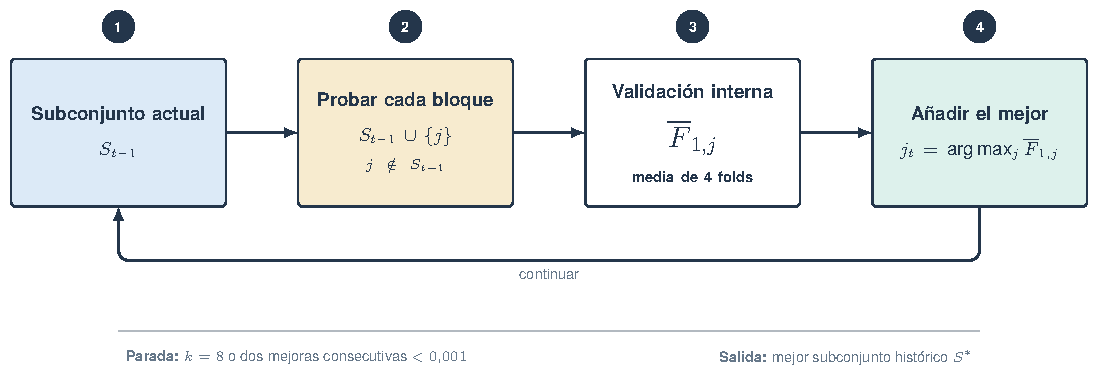
\includegraphics[width=\textwidth]{articulo/borrador_profesor/figures/gfs_pasos.pdf}
\caption{Mecanismo de Greedy Forward Selection sobre bloques completos. En cada paso se elige el bloque que maximiza el macro-F1 medio de la validación interna; el test externo se utiliza únicamente tras cerrar el subconjunto.}
\label{fig:gfs-pasos}
\end{figure}
\FloatBarrier

La Tabla~\ref{tab:config-gfs} concentra los parámetros de búsqueda, comunes a ambos clasificadores.

\begin{table}[!htbp]
\centering
\caption{Configuración de la selección GFS en el flujo general.}
\label{tab:config-gfs}
\fontsize{9}{11}\selectfont
\begin{tabular}{lp{8.4cm}}
\toprule
Elemento & Configuración \\
\midrule
Unidad de selección & Bloque completo generado por un extractor \\
Candidatos & Hasta 22 bloques candidatos \\
Criterio interno & Macro-F1 medio en cuatro folds estratificados y agrupados \\
Presupuesto & Hasta $k=8$ bloques \\
Parada & Dos mejoras consecutivas menores que 0,001; se devuelve el mejor paso histórico \\
Empates & Nombre del extractor, en orden determinista \\
Información excluida & Test externo y sus etiquetas durante toda la selección \\
\bottomrule
\end{tabular}
\end{table}
\FloatBarrier



\section{Perfil numérico de costos del piloto}
\begin{longtable}{@{}lr@{}}
\caption{Constantes del perfil del piloto, en ms por imagen. Son parámetros archivados del modelo de costos, no tiempos medidos del híbrido.}\label{tab:perfil-costos}\\
\toprule Bloque & $c_j$ ms\\ \midrule \endfirsthead
\toprule Bloque & $c_j$ ms\\ \midrule \endhead
\texttt{beitv2\_base\_final} & 12,22\\
\texttt{convnext\_v2\_t} & 15,68\\
\texttt{deit\_s} & 15,38\\
\texttt{densenet121} & 26,70\\
\texttt{dinov2} & 57,65\\
\texttt{dinov2\_large} & 177,30\\
\texttt{dinov2\_small} & 24,60\\
\texttt{drlbp} & 83,34\\
\texttt{efficientnet\_b0} & 14,39\\
\texttt{eva02\_base} & 19,32\\
\texttt{gabor} & 1029,21\\
\texttt{glcm} & 41,03\\
\texttt{hog} & 2,30\\
\texttt{lbp} & 50,61\\
\texttt{mae\_base} & 12,76\\
\texttt{resnet101} & 21,49\\
\texttt{resnet50} & 11,94\\
\texttt{rgb\_ngram\_svd} & 18,50\\
\texttt{siglip\_base} & 11,68\\
\texttt{swin\_t} & 21,42\\
\texttt{vgg16} & 12,05\\
\texttt{vit\_b16} & 26,85\\
\midrule Sobrecosto de política & 0,45\\
\bottomrule
\end{longtable}

El perfil es una colección de constantes archivadas, no una medición de extremo a extremo del híbrido. Incluye un sobrecosto fijo de política de 0,45 ms cuando existe rescate y excluye la latencia completa de sus múltiples SVM, transferencias y régimen de carga/residencia. Las mediciones de la cascada anterior no se transfieren automáticamente a esta implementación.
